\chapter{Design and Implementation}\label{Design and Implementation}

% BEGIN Sam's section

Figures \ref{block_diagram1.png} and \ref{block_diagram_final.png}shows the earliest high level design of the software for the system created in the first and last week of the project. In the early stages the options were kept open for specific implementation details. The early design essentially required software to be written for three devices; a client computer (GUI), an experiment server (control over access to the system, interface to the GUI, image processing) and an embedded device (controlling experiment hardware). 


As the revised diagram in Figure \ref{block_diagram_final.png} shows, to remove an extra layer of complexity it was decided to use a single device (the BeagleBone Black) to play the role of both the experiment server and the embedded device. From a software perspective, this eliminated the need for an entire layer of communication and synchronization. From a hardware perspective, use of the BeagleBone black instead of a Raspberry Pi removed the need to design or source analogue to digital conversion modules.

Another major design change which occurred quite early in the project is the switch from using multiple processes to running a single multithreaded process on the server. After performing some rudimentary testing (see Section \ref{Server Interface}) it became clear that a system of separate programs would be difficult to implement and maintain. Threads are similar to processes but are able to directly share memory, with the result that much less synchronisation is required in order to transfer information.

{\bf Note on filenames:} In the following, files and directories related to the server are located in the \href{https://github.com/szmoore/MCTX3420/tree/master/server}{server} directory, files related to the (currently used) GUI are in \href{https://github.com/szmoore/MCTX3420/tree/master/testing/MCTXWeb}{testing/MCTXWeb}, and files created for testing purposes are located in \href{https://github.com/szmoore/MCTX3420/tree/master/testing}{testing}. In the server there is nearly always an associated \texttt{.h} ``header'' file for each \texttt{.c} ``source'' file.

\begin{figure}[H]
	\centering
	\includegraphics[width=0.8\textwidth]{figures/block_diagram1.png}
	\caption{Block Diagram from Week 1 of the Project}
	\label{block_diagram1.png}
\end{figure}


\begin{figure}[H]
	\centering
	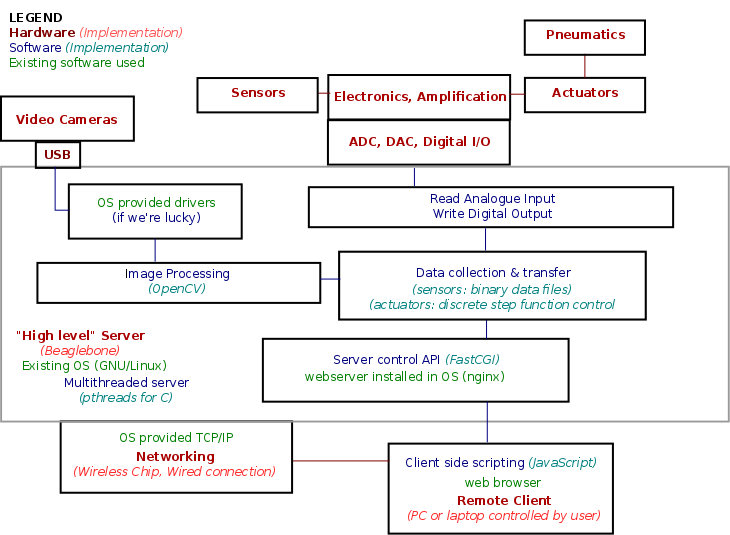
\includegraphics[width=0.8\textwidth]{figures/block_diagram_final.png}
	\caption{Block Diagram from Week 14 of the Project}
	\label{block_diagram_final.png}
\end{figure}

\section{Server Program}\label{Server Program}

\subsection{Threads and Sampling Rates}

The Server Program runs as a multithreaded process under a POSIX compliant GNU/Linux operating system\footnote{Tested on Debian and Ubuntu}. Each thread runs in parallel and is dedicated to a particular task; the three types of threads we have implemented are:
\begin{enumerate}
  \item Main Thread (Section \ref{Main Thread}) - Starts all other threads, accepts and responds to HTTP requests passed to the program by the HTTP server in the \funct{FastCGI_Loop} function (also see Section \ref{Server/Client Communication})
  \item Sensor Thread (Section \ref{Sensor Thread}) - Each sensor in the system is monitored by an individual thread running the \funct{Sensor_Loop} function.
  \item Actuator Thread (Section \ref{Actuator Thread}) - Each actuator in the system is controlled by an individual thread running the \funct{Actuator_Loop} function.
\end{enumerate}


In reality, threads do not run simultaneously; the operating system is responsible for sharing execution time between threads in the same way as it shares execution times between processes. Because the Linux kernel is not deterministic, it is not possible to predict when a given thread is actually running. This renders it impossible to maintain a consistent sampling rate, and necessitates the use of time stamps whenever a data point is recorded. 

Figure \ref{sample_rate_histogram.png} shows a distribution of times\footnote{The clock speed of the BeagleBone is around 1GHz\cite{bbb_specs}, which is fast enough to neglect the fact that recording the timestamp takes several CPU cycles.} between samples for a test sensor with the software sampling as fast as possible. Note the logarithmic $t$ axis. Although context switching clearly causes the sample rate to vary (\textcolor{green}{green}), the actual process of reading an ADC (\textcolor{red}{red}) using \funct{ADC_Read} (\gitref{server}{bbb_pin.c}) is by far the greatest source of variation.

It was not possible to obtain a real time Linux kernel for the BeagleBone. In theory, real time variants of the Linux kernel improve the reliability of sampling rates. However, testing on an amd64 laptop showed very little difference in the sampling time distribution when the real time Linux kernel was used.


\begin{figure}[H]
	\centering
	\includegraphics[width=0.8\textwidth]{figures/sample_rate_histogram.png}
	\caption{Sample Rate Histogram obtained from timestamps with a single test sensor enabled}
	\label{sample_rate_histogram.png}
\end{figure}


\subsection{Main Thread}\label{Main Thread}

The main thread of the process is responsible for transferring data between the server and the client through the Hypertext Transmission Protocol (HTTP). A library called FastCGI is used to interface with an existing webserver called nginx\cite{nginx}. This configuration and the format of data transferred between the GUI and the server is discussed in more detail Section \ref{Server/Client Communication}.

Essentially, the main thread of the process responds to HTTP requests. The GUI is designed to send requests periodically (e.g.: to update a graph) or when a user action is taken (e.g.: changing the pressure setting). When this is received, the main thread parses the request, the requested action is performed, and a response is sent. The GUI is then responsible for updating its appearance or alerting the user based on this response. Figure \ref{fastcgi-flow-chart.png} in Section \ref{API} gives an overview of this process.


\subsection{Sensor Threads}\label{Sensor Thread}

Figure \ref{sensor_thread.pdf} shows a flow chart for the thread controlling an individual sensor. This process is implemented by \verb/Sensor_Loop/ and associated helper functions.

All sensors are treated as returning a single floating point number when read. A \type{DataPoint} consists of a time stamp and the sensor value. \type{DataPoint}s are continuously saved to a binary file as long as the experiment is in process. An appropriate HTTP request (Section \ref{API}) will cause the main thread of the server program to respond with \type{DataPoint}s read back from the file. By using independent threads for reading data and transferring it to the GUI, the system does not rely on maintaining a consistent and synchronised network connection. This means that one the experiment is started with the desired parameters, a user can safely close the GUI or even shutdown their computer without impacting on the operation of the experiment.



As Figure \ref{sensor_thread.pdf} indicates, the processes of actually controlling sensor hardware has been abstracted out of the control loop. A \verb/Sensor/ structure is defined in \verb/sensor.h/ to represent a single sensor. When this structure is initialised, function pointers must be provided; these functions can then be called by \verb/Sensor_Loop/ as needed. All functions related to control over specific sensor hardware can be found in the files within the \verb/sensors/ sub directory.

Earlier versions of the software instead used a \verb/switch/ statement based on the \verb/Sensor/'s id number to determine how to obtain the sensor value. This was found to be difficult to maintain as the number and types of sensors supported by the software were increased.



\subsection{Actuator Threads}\label{Actuator Thread}

Actuators are controlled by threads in a similar way to sensors. Figure \ref{actuator_thread.pdf} shows a flow chart for these threads. This is implemented in \verb/Actuator_Loop/. Control over real hardware is separated from the main logic in the same way as sensors (relevant files are in the \verb/actuators/ sub directory). The use of threads to control actuators gives similar advantages in terms of eliminating the need to synchronise the GUI and server software.

The actuator thread has been designed for flexibility in how exactly an actuator is controlled. Rather than specifying a single value, the main thread initialises a structure that determines the behaviour of the actuator over a period of time. The current structure represents a simple set of discrete linear changes in the actuator value. This means that a user does not need to specify every single value for the actuator. The Actuator thread stores a value every time the actuator is changed which can be requested in a similar way to sensor data.



\subsection{Data Storage and Retrieval}

Each sensor or actuator thread stores data points in a separate binary file identified by the name of the device. When the main thread receives an appropriate HTTP request, it will read data back from the binary file. To allow for selection of a range of data points from the file, a binary search has been implemented. Functions related to data storage and retrieval are located in the \gitref{server}{data.h} and \gitref{server}{data.c} source files.

Several alternate means of data storage were considered for this project. Binary files were chosen because of the significant performance benefit after testing, and the ease with which data can be read from any location in file and converted directly into values. A downside of using binary files is that the server software must always be running in order to convert the data into a human readable format.



\subsection{Safety Mechanisms}

Given the inexperienced nature of the software team, the limited development time, and the unclear specifications, it is not wise to trust safety aspects of the system to software alone. It should also be mentioned that the correct functioning of the system is reliant not only upon the software written during this project, but also the many libraries which are used, and the operating system under which it runs. We found during development that many of the mechanisms for controlling BeagleBone hardware are unreliable and have unresolved issues; see the project wiki pages\cite{mctx3420_wiki} for more information. We attempted to incorporate safety mechanisms into the software wherever possible.

Sensors and Actuators should define an initialisation and cleanup function. For an actuator (e.g.: the pressure regulator), the cleanup function must set the actuator to a predefined safe value (in the case of pressure, atmospheric pressure) before it can be uninitialised. In the case of a software error or user defined emergency, the \funct{Fatal} function can be called from any point in the software; this will lead to the cleanup functions of devices being called, which will in turn lead to the pressure being set to a safe value. 

Sensors and Actuators are designed to include an optional \funct{sanity} function which will check a reading or setting is safe respectively. These checks occur whenever a sensor value is read or an actuator is about to be set. In the case of a sensor reading failing the sanity check, \funct{Fatal} is called immediately and the software shuts down the experiment. In the case of an actuator being set to an unsafe value the software will simply refuse to set the value.

It is recommended that the detection of signals (a mechanism in GNU/Linux by which a program can detect certain types of unexpected crashes) be investigated. This was attempted in early implementations; however difficulties were encountered because any thread can catch the signal and thus will not be able to execute its cleanup function, or in some cases, continue running after the rest of the program has stopped.

An alternative safety mechanism involves modification of the script that starts the server (\gitref{server}{run.sh}). This script is already able to detect when the program exits, and it should be possible to further extend this script to react accordingly to different exit codes.

\pagebreak
\begin{figure}[H]
	\centering
	\includegraphics[width=1.1\textwidth]{figures/sensor_thread.pdf}
	\caption{Flow chart for a sensor thread} 
	\label{sensor_thread.pdf}
\end{figure}
\pagebreak
\pagebreak
\begin{figure}[H]
	\centering
	\includegraphics[width=1.1\textwidth]{figures/actuator_thread.pdf}
	\caption{Flow chart for an actuator thread} 
	\label{actuator_thread.pdf}
\end{figure}


\section{Hardware Interfacing}\label{Hardware Interfacing}

Figure \ref{pinout.pdf} shows the pin out diagram of the BeagleBone Black. There are many contradictory pin out diagrams available on the internet; this figure was initially created by the software team after trial and error testing with an oscilloscope to determine the correct location of each pin. Port labels correspond with those marked on the BeagleBone PCB. The choice of pin allocations was made by the electrical team after discussion with software when it became apparent that some pins could not be controlled reliably.




\subsection{Sensors}

Code to read sensor values is located in the \gitref{server}{sensors} subdirectory. With the exception of the dilatometer (discussed in Section \ref{Image Processing}), all sensors used in this project produce an analogue output. After conditioning and signal processing, this arrives at an analogue input pin on the BeagleBone as a signal in the range $0\to1.8\text{V}$. The sensors currently controlled by the software are:

\begin{itemize}
	\item {\bf Strain Gauges} (x4) \gitref{server}{sensors/strain.c}

	To simplify the amplifier electronics, a single ADC is used to read all strain gauges. GPIO pins are used to select the appropriate strain gauge output from a multiplexer. A mutex is used to ensure that no two strain gauges can be read simultaneously.


	\item {\bf Pressure Sensors} (x3) \gitref{server}{sensors/pressure.c}

	 There are two high range pressure sensors and a single low range pressure sensor; all three are read independently
	\item {\bf Microphone} (x1) \gitref{server}{sensors/microphone/c}

	The microphone's purpose is to detect the explosion of a can. This sensor was given a low priority, but has been tested with a regular clicking tone and found to register spikes with the predicted frequency (~1.5Hz).
	\item {\bf Dilatometer} (x2) - \gitref{server}{sensors/dilatometer.c} See Section \ref{Image Processing}
\end{itemize}

Additional sensors can be added and enabled through use of the \funct{Sensor_Add} function in \funct{Sensor_Init} in the file \gitref{server}{sensor.c}.

The function \funct{Data_Calibrate} located in \gitref{server}{data.c} can be used for interpolating calibration. The pressure sensors and microphone have been calibrated in collaboration with the Sensors Team; however only a small number of data points were taken and the calibration was not tested in detail. We would recommend a more detailed calibration of the sensors for future work.

\subsection{Actuators}

Code to set actuator values is located in the \gitref{server}{actuators} subdirectory. The following actuators are (as of writing) controlled by the software and have been successfully tested in collaboration with the Electronics and Pneumatics teams. Additional actuators can be added and enabled through use of the \funct{Actuator_Add} function in \funct{Actuator_Init} in the file \gitref{server}{actuator.c}.

\subsubsection{Relay Controls} \gitref{server}{actuators/relay.c}

The electrical team employed three relays for control over digital devices. The relays are switched using the GPIO outputs of the BeagleBone Black.

\begin{itemize}
	\item Can select - Chooses which can can be pressurised (0 for strain, 1 for explode)
	\item Can enable - Allows the can to be pressurised (0 for vent, 1 for enable)
	\item Main enable - Allows pressure to flow to the system (0 for vent, 1 for enable) and can be used for emergency venting
\end{itemize}

The use of a ``can select'' and ``can enable'' means that it is not a software problem to prevent both cans from simultaneously being pressurised. This both simplifies the software and avoids potential safety issues if the software were to fail.


\subsubsection{PWM Outputs}

A single PWM output is used to control a pressure regulator (\gitref{server}{actuators/pregulator.c}). The electrical team constructed an RC filter circuit which effectively averages the PWM signal to produce an almost constant analogue output. The period of the PWM is $2\text{kHz}$. This actuator has been calibrated, which allows the user to input the pressure value in kPa rather than having to control the PWM duty cycle correctly.


\begin{figure}[H]
	\centering
	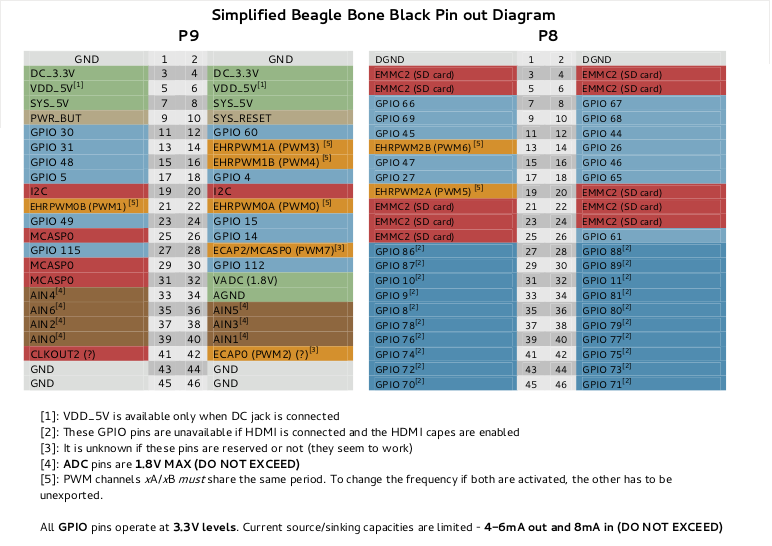
\includegraphics[angle=90,width=1.0\textwidth]{figures/pinout.pdf}
	\caption{Pinout Table} 
	\label{pinout.pdf}
\end{figure}


\section{Authentication Mechanisms}\label{Authentication Mechanisms}

The \funct{Login_Handler} function (\gitref{server}{login.c}) is called in the main thread when a HTTP request for authentication is received (see Section \ref{Communication}). This function checks the user's credentials and will give them access to the system if they are valid. Whilst we had originally planned to include only a single username and password, changing client requirements forced us to investigate many alternative authentication methods to cope with multiple users.

Several authentication methods are supported by the server; the method to use can be specified as an argument when the server is started.
\begin{enumerate}
  \item {\bf Unix style authentication}


  Unix like operating systems store a plain text file (/etc/shadow) of usernames and encrypted passwords\cite{shadow}. To check a password is valid, it is encrypted and then compared to the stored encrypted password. The actual password is never stored anywhere. The /etc/shadow file must be maintained by shell commands run directly from the BeagleBone. Alternatively a web based system to upload a similar file may be created.

  \item {\bf Lightweight Directory Access Protocol (LDAP)}

  LDAP\cite{ldap, ldap_man} is a widely used data base for storing user information. A central server is required to maintain the LDAP database; programs running on the same network can query the server for authentication purposes.

  The UWA user management system (Pheme) employs an LDAP server for storing user information and passwords. The software has been designed so that it can interface with an LDAP server configured similarly to the server on UWA's network. Unfortunately we were unable to gain permission to query this server. However an alternative server could be setup to provide this authentication mechanism for our system.


  \item {\bf MySQL Database}

        MySQL\cite{mysql} is a popular and free database system that is widely used in web applications. The ability to search for a user in a MySQL database and check their encrypted password was added late in the design as an alternative to LDAP. There are several existing online user management systems which interface with a MySQL database, and so it is feasible to employ one of these to maintain a list of users authorised to access the experiment. UserCake\cite{UserCake} is recommended, as it is both minimalistic and open source, so can be modified to suit future requirements. We have already begun integration of the UserCake system into the project, however a great deal of work is still required.


  MySQL and other databases are vulnerable to many different security issues which we did not have sufficient time to fully explore. Care should be taken to ensure that all these issues are addressed before deploying the system.


\end{enumerate}

% END Sam's section


\section{Server/Client Communication}\label{Server/Client Communication}

% BEGIN Jeremy's section

This section describes the methods and processes used to communicate between the server and client. For this system, client-server interaction is achieved completely over the internet, via standard HTTP web requests with TLS encryption. In other words, it has been designed to interact with the client over the internet, {\bf completely through a standard web browser} (Figure \ref{client_request_flowchart.png}). No extra software should be required from the client. Detailed reasons for this choice are outlined in Section \ref{Alternative Communication Technologies}

\begin{figure}[H]
	\centering
	\includegraphics[width=0.8\textwidth]{figures/client_request_flowchart.png}
	\caption{High level flow chart of a client request to server response} 
	\label{client_request_flowchart.png}
\end{figure}

\subsection{Web server}

Web requests from a user have to be handled by a web server. For this project, the nginx\cite{nginx} webserver has been used, and acts as the frontend of the remote interface for the system. As shown in Figure \ref{client_request_flowchart.png}, all requests to the system from a remote client are passed through nginx, which then delegates the request to the required subsystem as necessary. 

In particular, nginx has been configured to:
\begin{enumerate}
	\item Use TLS encryption (HTTPS)
	\item Forward all HTTP requests to HTTPS requests (force TLS encryption)
	\item Display the full sever program logs if given \api{log} as the address
	\item Display the warning and error logs if given \api{errorlog} as the address
	\item Forward all other requests that start with \api{} to the server program (FastCGI)
	\item Process and display PHP files (via PHP-FPM) for UserCake
	\item Try to display all other files like normal (static content; e.g the GUI)
\end{enumerate}

Transport Layer Security (TLS) encryption, better known as SSL or HTTPS encryption has been enabled to ensure secure communications between the client and server. This is primarily important for when user credentials (username / password) are supplied, and prevents what is called ``man-in-the-middle'' attacks. In other words, it prevents unauthorised persons from viewing such credentials as they are transmitted from the client to the server. 

As also mentioned in Section \ref{Authentication Mechanisms} this system also runs a MySQL server for the user management system, UserCake. This kind of server setup is commonly referred to as a LAMP (Linux, Apache, MySQL, PHP) configuration\cite{lamp}, except in this case, nginx has been used in preference to the Apache web server. 

Nginx was used as the web server because it is well established, lightweight and performance oriented. It also supports FastCGI by default, which is how nginx interfaces with the server program. Realistically, any well known web server would have sufficed, such as Apache or Lighttpd, given that this is not a large scale service.

\subsection{FastCGI}

Nginx has no issue serving static content --- that is, just normal files to the user. Where dynamic content is required, as is the case for this system, another technology has to be used, which in this case is FastCGI.

FastCGI is the technology that interfaces the server program that has been written with the web server (nginx). As illustrated in Figure \ref{client_request_flowchart.png}, there is a ``FastCGI layer'', which translates web requests from a user to something which the server program can understand, and vice versa for the response. 

\subsection{Server API - Making Requests}\label{API}

From the client side, the server interface is accessed through an Application Programming Interface (API). The API forms a contract between the client and server; by requesting a URL of a predetermined format, the response will also be of a predetermined format that the client can use.

\begin{figure}[H]
	\centering
	\includegraphics[width=0.9\textwidth]{figures/fastcgi-flow-chart.png}
	\caption{Flow chart of a client request being processed (within the server program). Relevant files are \gitref{server}{fastcgi.c} and \gitref{server}{fastcgi.h}.} 
	\label{fastcgi-flow-chart.png}
\end{figure}

In the case of the server API designed, requests are formatted as such: 

\url{https://host/api/module?key1=value1&key2=value2...&keyN=valueN} (where \verb/host/ is replaced with the IP address or hostname of the server).


The API consists of modules accepting arguments (specified as key-value pairs), depending on what that module (Figure \ref{modules}) does. For example, to query the API about basic information (running state, whether the user is logged in etc), the following query is used:

\url{https://host/api/identify}

The server will then respond with this information. In this case, the identify module does not require any arguments. However, it can accept two optional arguments, \texttt{sensors} and \texttt{actuators}, which makes it give extra information on the available sensors and actuators present. This makes the following queries possible:

\begin{itemize}
	\item \url{https://host/api/identify?sensors=1}
	\item \url{https://host/api/identify?actuators=1}
	\item \url{https://host/api/identify?sensors=1&actuators=1}
\end{itemize}

These give information on the sensors, actuators, or both, respectively. For other modules some parameters may be required, and are not optional.
This form of an API was chosen because it is simple to use, and extremely easy to debug, given that these requests can just be entered into any web browser to see the result. The request remains fairly human readable, which was another benefit when debugging the server code. 

Keeping the API format simple also made it easier to write the code that parsed these requests. All API parsing and response logic lies in \gitref{server}{fastcgi.c}. The framework in \gitref{server}{fastcgi.c} parses a client request and delegates it to the relevant module handler. Once the module handler has sufficiently processed the request, it creates a response, using functions provided by \gitref{server}{fastcgi.c} to do so. 

This request handling code went through a number of iterations before the final solution was reached. Changes were made primarily as the number of modules grew, and as the code was used more. 

One of the greatest changes to request handling was with regards to how parameters were parsed. Given a request of: \url{http://host/api/actuators?name=pregulator\&start_time=0\&end_time=2}, The module handler would receive as the parameters \texttt{name=pregulator\&start_time=0\&end_time=2}. This string had to be split into the key/value pairs, so the function \funct{FCGI_KeyPair} being made.

With increased usage, this was found to be insufficient. \funct{FCGI_ParseRequest} was created in response, and internally uses \funct{FCGI_KeyPair}, but abstracts request parsing greatly. In essence, it validates the user input, rejecting anything that doesn't match a specified format. If it passes this test, it automatically populates variables with these values. The \funct{IndentifyHandler} module handler in \gitref{server}{fastcgi.c} is a very good example of how this works. 

\begin{figure}[H]
	\centering
	\begin{tabular}{llll}
		{\bf API} & {\bf File} & {\bf Function} & {\bf Purpose} \\
		\api{identify} & \gitref{server}{fastcgi.c} & \funct{IdentifyHandler} & Provide system information \\
		\api{sensors} & \gitref{server}{sensor.c} & \funct{Sensor_Handler} & Query sensor data points or set sampling rate\\
		\api{actuators} & \gitref{server}{actuator.c} & \funct{Actuator_Handler} & Set actuator values or query past history \\
		\api{image} & \gitref{server}{image.c} & \funct{Image_Handler} & Return image from a camera (See Section \ref{Image Processing}) \\
		\api{control} & \gitref{server}{control.c} & \funct{Control_Handler} & Start/Stop/Pause/Resume the Experiment \\
		\api{bind} & \gitref{server}{login.c} & \funct{Login_Handler} & Attempt to login to the system (See Section \ref{Cookies})\\
		\api{unbind} & \gitref{server}{login.c} & \funct{Logout_Handler} & If logged in, logout.
	\end{tabular}
	\caption{Brief description of the modules currently implemented by the server.}
	\label{modules}
\end{figure}

\subsection{Server API - Response Format}

The server API primarily generates JSON responses to most requests. This was heavily influenced by what the GUI would be programmed in, being JavaScript. This particular format is parsed easily in JavaScript, and is easily parsed in other languages too. 

A standard JSON response looks like such:

\begin{figure}[H]
	\centering
\begin{verbatim}
{
    "module" : "identify",
    "status" : 1,
    "start_time" : 614263.377670876,
    "current_time" : 620591.515903585,
    "running_time" : 6328.138232709,
    "control_state" : "Running",
    "description" : "MCTX3420 Server API (2013)",
    "build_date" : "Oct 24 2013 19:41:04",
    "api_version" : 0,
    "logged_in" : true,
    "user_name" : "_anonymous_noauth"
}
\end{verbatim} 
	\caption{A standard response to querying the \api{identify} module}
	\label{fastcgi.c-flow-chart.pdf}
\end{figure}

A JSON response is the direct representation of a JavaScript object, which is what makes this format so useful. For example if the JSON response was parsed and stored in the object \var{data}, the elements would be accessible in JavaScript through \var{data.module} or \var{data.status}.

To generate the JSON response from the server program, \gitref{server}{fastcgi.c} contains a framework of helper functions. Most of the functions help to ensure that the generated output is in a valid JSON format, although only a subset of the JSON syntax is supported. Supporting the full syntax would overcomplicate writing the framework while being of little benefit. Modules can still respond with whatever format they like, using \funct{FCGI_JSONValue} (aka. \funct{FCGI_PrintRaw}), but lose the guarantee that the output will be in a valid JSON format. 

Additionally, not all responses are in the JSON format. In specific cases, some module handlers will respond in a more suitable format. For example, the image handler will return an image (using \funct{FCGI_WriteBinary}); it would make no sense to return anything else. On the other hand, the sensor and actuator modules will return data as tab-separated values, if the user specifically asks for it (e.g.: using \url{https://host/api/sensors?id=X&format=tsv})

\subsection{Server API - Cookies}\label{Cookies}

The system makes use of HTTP cookies to keep track of who is logged in at any point. The cookie is a small token of information that gets sent by the server, which is then stored automatically by the web browser. The cookie then gets sent back automatically on subsequent requests to the server. If the cookie sent back matches what is expected, the user is `logged in'. Almost all web sites in existence that has some sort of login use cookies to keep track of this sort of information, so this method is standard practice. 
In the server code, this information is referred to as the `control key'. A control key is only provided to a user if they provide valid login credentials, and no one else is logged in at that time. 

The control key used is the SHA-1 hash of some randomly generated data, in hexadecimal format. In essence, this is just a string of random numbers and letters that uniquely identifies the current user.

Initially, users had to pass this information as another key-value pair of the module parameters. However, this was difficult to handle, both for the client and the server, which was what precipitated the change to use HTTP cookies.

\subsection{Client - JavaScript and AJAX Requests}

JavaScript forms the backbone of the web interface that the clients use. JavaScript drives the interactivity behind the GUI and enables the web interface to be updated in real-time. Without JavaScript, interactivity would be severely limited, which would be a large hindrance to the learning aspect of the system. 

To maintain interactivity and to keep information up-to-date with the server, the API needs to be polled at a regular interval. Polling is necessary due to the design of HTTP; a server cannot ``push'' data to a client, the client must request it first. To be able to achieve this, code was written in JavaScript to periodically perform what is termed AJAX requests. 

AJAX requests are essentially web requests made in JavaScript that occur ``behind the scenes'' of a web page. By making such requests in JavaScript, the web page can be updated without having the user refresh the web page, thus allowing for interactivity and a pleasant user experience.

Whilst AJAX requests are possible with plain JavaScript, the use of the jQuery library (see Section \ref{jQuery}) greatly simplifies the way in which requests can be made and interpreted.

\section{Alternative Communication Technologies}\label{Alternative Communication Technologies}

This section attempts to explain the reasoning behind the communication method chosen. This choice was not trivial, as it had to allow for anyone to remotely control the experiment, while imposing as little requirements from the user as possible. These requirements can be summarised by:
\begin{enumerate}
	\item A widely available, highly accessible service should be used, to reach as many users as possible
	\item Communication between client and server should be fairly reliable, to maintain responsiveness of the remote interface
	\item Communication should be secured against access from unauthorised persons, to maintain the integrity of the system
\end{enumerate}

To satisfy the first criteria, remote control via some form of internet access was the natural choice. Internet access is widely established and highly accessible, both globally and locally, where it can be (and is) used for a multitude of remote applications. One only needs to look as far as the UWA Telelabs project for such an example, having been successfully run since 1994 \cite{telelabs}.

Internet communications itself is complex, and there is more than one way to approach the issue of remote control. A number of internet protocols exist, where the protocol chosen is based on the needs of the application. Arguably most prevalent is the Hypertext Transfer Protocol (HTTP)\cite{rfc2616} used in conjunction with the Transmission Control Protocol (TCP) - to distribute web pages and related content across the internet. Other protocols exist, but are less widely used. Even custom protocols can be used, but that comes at the cost of having to build, test and maintain an extra component of software that likely has no benefit over pre-existing systems.

As a result, being able to control the system via a web page and standard web browser seemed the most logical choice, which was why it was used in the final design. Firstly, by designing the system to be controlled from a web page, the system becomes highly accessible, given that where internet access is present, the presence of a web browser is almost guaranteed. Nothing else from the client is required. 

Secondly, setup and maintenance for the server is less involved, given that there is a wide range of pre-existing software made just for this purpose. Many features of the web browser can also be leveraged to the advantage of the system --- for example, communications between the client and server can be quite easily secured using Transport Layer Security (TLS, previously known as Secure Sockets Layer or SSL).

Thirdly, reliability of the communications is better guaranteed by using such existing technology, which has been well tested and proven to work of its own accord. While internet access itself may not always be fully reliable, the use of such protocols and correct software design allows for a fair margin of robustness towards this issue. For example, TCP communications have error checking methods built-in to the protocol, to ensure the correct delivery of content. Similarly, HTTP has been designed with intermittent communications to the client in mind\cite{rfc2616}.

\subsection{Server Interface} \label{Server Interface}
Other options were explored apart from FastCGI to implement the server interface. Primarily, it had to allow for continuous sensor/actuator control independent of user requests, which may be intermittent.

\begin{figure}[H]
	\centering
	\includegraphics[width=0.8\textwidth]{figures/cgi.png}
	\caption{Block Diagram of a request to a CGI Application} 
	\label{cgi.png}
\end{figure}

Initially, a system known as ``Common Gateway Interface'', or CGI was explored. However, CGI based software is only executed when a request is received (Figure \ref{cgi.png}), which makes continuous control and logging over the sensors and actuators unfeasible. 

\begin{figure}[H]
	\centering
	\includegraphics[width=0.8\textwidth]{figures/custom_webserver.png}
	\caption{Block Diagram of a request to a custom web server} 
	\label{custom_webserver.png}
\end{figure}

Another system considered was to build a custom web server (Figure \ref{custom_webserver.png}) that used threading, integrating both the control and web components. This option was primarily discarded because it was inflexible to supporting extended services like PHP and TLS encryption. See \href{https://github.com/szmoore/MCTX3420/issues/6}{Issue 6}\cite{github_issues} on GitHub for more information.

\begin{figure}[H]
	\centering
	\includegraphics[width=0.8\textwidth]{figures/fastcgi.png}
	\caption{Block Diagram of a request to a FastCGI application} 
	\label{fastcgi.png}
\end{figure}

In comparison, FastCGI (Figure \ref{fastcgi.png}) can be seen as the ``best of both worlds''. As mentioned previously, it is a variant of CGI, in that it allows some software to respond to web requests. The key difference is that with FastCGI, the program is continuously run independent of any web requests. This overcomes the issues faced with either using CGI or a custom web server; continuous control can be achieved while also not having to worry about the low-level implementation details a web server.



\subsection{Recommendations for Future Work}

\begin{enumerate}
	\item A self-signed TLS certificate has been used, as it is free. It is equally secure as any, but users will get a security warning when accessing the web site. A proper TLS certificate signed by a trusted certificate authority should be used instead.
	\item Consider expanding the framework of JSON functions to simplify creating a response. 
	\item Consider using X-Accel-Redirect along with UserCake (Section \ref{Authentication Mechanisms}) to make a finer-grained access control system to information such as the system logs
\end{enumerate}

\section{BeagleBone Configuration}\label{BeagleBone Configuration}

\subsection{Operating system}
The Beaglebone has been configured to use the Ubuntu operating system. The original operating system was Angstrom, which was unsuitable because it lacked a number of software packages required. Detailed instructions on how to install this operating system exist on the project wiki\cite{mctx3420_wiki}.

In particular, Ubuntu 13.04 running Linux kernel 3.8.13-bone28 was used, which is essentially the latest version available to date for this platform. Normally an older, more tested version is recommended, especially in a server environment. However, the BeagleBone Black is a relatively new device, and it was found that a lot of the drivers simply do not work well on older versions.

Specifically, there was much grief over getting the pins to function correctly, especially for PWM output. Lacking any great documentation, much trial and error was spent determining the best configuration. The BeagleBone Black uses what is termed a ``device tree'' \cite{beaglebone3.8, devicetreetutorial} and ``device tree overlays'' to dynamically determine what each pin does. This is because each pin can have more than one function, so a ``device tree overlay'' determines what it does at any one point. However, this also complicates matters, since what pins do essentially have to be loaded at runtime. 

PWM control in particular took many hours to achieve, which was not helped by a lot of conflicting information available online. As a result, the primary tool used to correctly determine proper PWM control was the use of a cathode ray oscilloscope. Quite briefly, it was found that certain actions had to be performed in a very specific order to make PWM control available. The wiki goes into more detail on the issues found.

Getting the cameras to work on the BeagleBone was another major issue faced. After much testing, it was simply found that the cameras could only work on the latest version of the operating system. On anything else, only low resolution captures of around 352x288 pixels could be achieved.

Finally, it should be noted that USB hot-plugging does not work on the BeagleBone. This means that the cameras have to be plugged in before booting the BeagleBone. Upgrading to a newer kernel (when it exists) should solve this issue.


\subsection{Required software}
A number of packages are required to compile the code:
\texttt{nginx spawn-fcgi libfcgi-dev gcc libssl-dev make libopencv-dev valgrind libldap2-dev mysql-server libmysqlclient-dev php5 php5-gd php5-fpm php5-mysqlnd}

These packages should be installed with the command \texttt{apt-get install}.

\subsection{Required configurations}
Many components need to be configured correctly for the server to work. In particular, these configurations relate to the web server, nginx, as well as logging software used, rsyslog. Executing \gitref{server-configs}{install.sh} as root should install all the required configuration files to run the server correctly.

% END Jeremy's section

\subsection{Logging and Debugging}

The function \funct{Log} located in \gitref{server}{log.c} is used extensively throughout the server program for debugging, warning and error reporting. This function uses syslog to simultaneously print messages to the \texttt{stderr} output stream of the program and log them to a file, providing a wealth of information about the (mal)functioning of the program. As discussed in Section \ref{API}, the logs may be also be viewed by a client using the server API.

For more low level debugging, ie: detecting memory leaks, uninitialised values, bad memory accesses, etc, the program \texttt{valgrind}\cite{valgrind} was frequently used.



\section{Image Processing}\label{Image Processing}


% BEGIN Callum's section


The system contains two USB cameras, the Logitech C170\cite{logitechC170} and the Kaiser Baas KBA03030 (microscope)\cite{kaiserbaasKBA03030}.  The Logitech camera will be used to record and stream the can being pressurized to explode.  The microscope will be used to measure the change in width in the can. 

\subsection{OpenCV}

For everything related to image acquisition and processing we decided to use a library called OpenCV\cite{OpenCV}. OpenCV uses the capture structure to connect with cameras, and stores the data in \type{IplImage} structures and the newer \type{CvMat} structure.  As in C we cannot transfer the data straight to \type{CvMat} we need to convert from \type{IplImage} to \type{CvMat}.  There are two main functions required for use with the camera.  We need to be able to stream images to the user interface and use the microscope as a dilatometer, returning the rate of expansion of the can.  


\subsection{Image Streaming}
The image streaming is done through the function file \gitref{server}{image.c} and the header \gitref{server}{image.h}. There are only 2 functions in \gitref{server}{image.c}, both of which are externally accessible by the rest of the system.

 The \funct{Image_Handler} function handles requests from the server.  The parameters required for taking the image, such as the camera ID, width and height are determined by calling \funct{FCGI_ParseRequest} (see \gitref{server}{fastcgi.h} and \gitref{server}{fastcgi.c}) using the parameter string passed to the function.

The function \funct{Camera_GetImage} in \gitref{server}{image.c} is used to capture a frame on the camera from the ID given by \var{num}.  As we cannot have 2 camera structures open at once, we use a mutex to ensure the function execute concurrently. We check to see if \var{num} is equivalent to the previous camera ID, if so we do not need to close the capture in order to recreate the connection with the new camera, which takes time.  These considerations are currently redundant as the decision was made to only have one camera connected at a time, which was mainly due to power and bandwidth issues.  However the code was implemented to allow for further development.  If more than 2 cameras are ever connected, then the allowable upper bound for \var{num} will need to be increased to $n-1$ (where $n$ is the number of cameras connected to the system).  

After capturing the image we encode the \type{IplImage}, which passes back an encoded \type{CvMat}. The image is then returned back to the web browser via \funct{FCGI_WriteBinary}, where it can be displayed.  

\subsection{Dilatometer}

The dilatometer algorithm is used to determine the rate of expansion of the can. The relevant functions are declared in \gitref{server}{sensors/dilatometer.c} and \gitref{server}{sensors/dilatometer.h}. When an experiment is started, \funct{Dilatometer_Init} is  executed.  This creates all the necessary structures and sets the initial value of \var{lastPosition}, which is a static variable that stores the last edge found.

As the \funct{Camera_GetImage} function in \gitref{server}{image.c} is external, it can be accessed from \gitref{server}{sensors/dilatometer.c}.  This was done so that both the dilatometer and the image stream can gain access to the camera.  The \type{IplImage} returned is converted to the \type{CvMat} structure \var{g_srcRGB}.  This \type{CvMat} structure is then passed to a function, \funct{CannyThreshold}.  In this function, a series of steps are taken to extract an image containing only the edges.  First we use \funct{cvCvtColor} to convert the \type{CvMat} file to a grayscale image.  The image is then blurred using the \funct{cvSmooth} function, which we pass the parameters \var{CV_GAUSSIAN} and \var{BLUR}, so  we use a Gaussian blur with a kernel of size \var{BLUR} (defined in \gitref{server}{sensors/dilatometer.h}).  The blurred file is then passed to the OpenCV Canny Edge detector.  

The Canny Edge algorithm\cite{OpenCV_Canny} determines which pixels are ``edge'' pixels through a series of steps.  The algorithm applies the Sobel operator in the x and y directions using \var{KERNELSIZE} for the size of the kernel.  The result of this gives the gradient strength and direction. The direction is rounded to 0, 45, 90 or 135 degrees. Non-maximum suppression is then used to remove any pixels not considered to be part of an edge.  The pixels left are then put through the hysteresis step.  If the gradient of the pixel is higher than the upper threshold (in our algorithm denoted by \var{LOWTHRESHOLD*RATIO}) then the pixel is accepted as an edge.  If it is below the lower threshold (i.e. \var{LOWTHRESHOLD}) then the pixel is disregarded.  The remaining pixels are removed unless that is connected to a pixel above the upper threshold (Canny Edge Detector). The defined values in the header file can be altered to improve accuracy.

The \funct{CannyThreshold} function fills the \type{CvMat} \var{g_edges} structure with the current image edge (i.e. an image containing only pixels considering to be edges, see Figure \ref{canny_demo} (C-F)). The code then finds the location of the line.  It does this by sampling a number of rows, determined by the number of samples and the height of the image, finding the pixel/s in the row considered to be an edge.  The algorithm then takes the average position of these pixels.  The average position over all rows sampled then determines the actual edge position.  The rows sampled are evenly spaced over the height of the image.  If a row does not contain an edge, then it will not be included in the average.  If a blank image goes through, or the algorithm has a low number of samples and does not pick up an edge, then the function will return false and the data point will not be recorded.

Once the edge is found, we will either return the position of the edge, if the \var{DIL_POS} ID is set. It needs to be noted that this will only show the change in position of one side of the can.  If the \var{DIL_DIFF} ID is set then the value will be set to the difference between the current position and the last position, multiplied by \var{SCALE} and 2.  We need to multiply by 2 as we are only measuring the change in width to one side of the can, however we must assume that the expansion is symmetrical.  The scale will be used to convert from pixels to $\mu$m (or a more suitable scale).  Currently the scale is set to 1, as the dilatometer has not been calibrated, thus we are only measuring the rate of change of pixels (which is arbitrary). The static variable, \var{lastPosition}, is then set to determine the next change in size.  If the difference is negative, then the can is being compressed or is being depressurized. 
The rate of expansion can then be determined from the data set.  As the system does not have a fixed refresh rate, however each data point is time-stamped.  If the data is the edge position, then plotting the derivative of the time graph will show the rate of expansion over time.

\subsection{Design Considerations}

\subsubsection{OpenCV}

OpenCV was chosen as the image processing library primarily due to it being open source and widely used in image processing tasks.  
One thing to note however is the documentation for OpenCV for the language C is quite difficult to follow.  This is mainly due to the fact that the source (despite originally being written for C) is now written primarily for use in C++, thus the documentation and some of the newer functionality is tailored more for C++.  This caused some difficulty in writing the code for C as not all C++ functionality was available for C, or was included in a different or outdated fashion. 

\subsubsection{Memory Management}

An initial problem we faced when coding in OpenCV was memory leaks.  Our simple program to take an image and save it to file was causing us to lose approximately 18Mb, which is unacceptable and would cause issues in the long term.  After researching the issue we found that we were not properly releasing the structure dealing with storing the image for the data, \type{IplImage}.  For example we were using:
\begin{lstlisting}
	cvReleaseImage(&frame);
\end{lstlisting}
When the correct release function is actually:
\begin{lstlisting}
	cvReleaseImageHeader(&frame);
\end{lstlisting}

Another thing to note was that releasing one of the \type{CvMat} structures (\verb/g_srcRGB/) during the cleanup of the dilatometer module, a \verb/NULL/ pointer exception was returned and the program execution stopped.  The reason for this is unknown, but the other \type{CvMat} structures appear to be released properly. For now we simply removed this release; however the cause should be looked into.

\subsubsection{Dilatometer}
The dilatometer code went through a few iterations.  Originally we were informed by the Sensors Team that the camera would be watching the can, rather than object attached to the can.  Thus our original algorithms were revolved around finding the actual width and change in width of the can.

Originally we designed the algorithm to find the edge of the can via the pixel thresholds.  By finding the average position of the pixels below a certain threshold (as ideally you would have a dark can on a light background to create a contrast for the edge). This would already give a fairly inaccurate result, as it assumes a relatively sharp intensity gradient.  Even with little noise the system would have accuracy issues.

To increase the accuracy in finding the edge, we considered the Canny Edge theorem.  We wrote the algorithm to find all points above a certain threshold and take the average of these, considering this as an edge.  We then scanned through the rest of the image until the next edge was found and do the same.  The width of the can is found by taking the difference of the two locations. A test algorithm was also written to generate the egdes in order to test the algorithm.  The function (\funct{Dilatometer_TestImage}/, which is still located within \gitref{server}{sensors/dilatometer.c}) generated two edges, with an amount of noise.  The edges were created by taking an exponential decay around the edge and adding (and subtracting) a random noise from the expected decay.  The edges where then moved outwards using a for loop. From Figure \ref{canny_edges.png}, it can be seen how effective the algorithm was for a system with negligible noise, as it gave negligible percentage error.  However with increasing levels of noise we notice a considerable increase in inaccuracy (Figure \ref{canny_edges_noise.png}).  



\begin{figure}[H]
	\centering
	\includegraphics[width=0.9\textwidth]{figures/canny_edges.png}
	\caption{Output of canny edge algorithm applied to generated edges} 
	\label{canny_edges.png}
\end{figure}

\begin{figure}[H]
	\centering
	\includegraphics[width=0.9\textwidth]{figures/canny_edges_noise.png}
	\caption{Output of canny edge algorithm applied to generated edges with generated noise} 
	\label{canny_edges_noise.png}
\end{figure}

After the Sensors Team relayed that they were now attaching something to the can in order to measure the change position, we decided to simply stick with the Canny Edge algorithm and implement something similar to what we had in my previous testing.  The images in Figure \ref{canny_demo} shows the progression of the image through the algorithm. Figure \ref{canny_demo}A shows the original image, whereas \ref{canny_demo}B shows the blurred (with a BLUR value of 9) gray scale image.  Whereas Figure \ref{canny_demo}C shows the image after going through the Canny Edge algorithm with a low threshold of 35 and the location of the determined edge superimposed on top.    

Figures \ref{canny_demo}D, \ref{canny_demo}E and \ref{canny_demo}F all have the same input image (however different to \ref{canny_demo}A).  Figure \ref{canny_demo}D had a blur of 5 and a low threshold value of 40, \ref{canny_demo}E had a blur of 9 and a low threshold value of 35, and \ref{canny_demo}F had a blur of 7 and a low threshold of 36.  It can be seen how tweaking the values can remove outliers, as Figure \ref{canny_demo}D is skewed to the right due to theincreased number of outliers.  From Figure \ref{canny_demo}E it can be seen that despite there being no points in the edge in the top half of the image, the edge has still been accurately determined.  

The testing done shows that given a rough edge with few outliers an edge can be determined, however there is an obvious degree of inaccuracy the greater the variance of the edge. The best solution to this however does not lie in software.  If an edge was used that was straight even at that magnification with a good contrast then the results would be much more accurate (i.e. the accuracy of the dilatometer is currently more dependent on the object used than the software). 
  

\subsubsection{Interferometer}
Earlier in the semester we were informed by the Sensors Team that instead of a dilatometer we would be using an interferometer.  The algorithm for this was written and tested; it is currently still located in the file \gitref{server}{interferometer.c} and header \gitref{server}{interferometer.h}. However development of the algorithm ceased after the sensors team informed us that the interferometer would no longer be implemented.

\subsection{Further Design Considerations}

\begin{itemize}
	\item During testing we noted a considerable degree of lag between the image stream and reality. Further testing can be done to determine the causes and any possible solutions.
	\item A function to help calibrate the dilatometer should be created
	\item The algorithm should be tested over an extended period of time checking for memory leak issues caused by OpenCV.
	\item Possibly modify the code to allow the parameters used in the Canny Edge algorithm to be modified in real time so the user can try and maximize the accuracy of the results.  The image with the edge superimposed on it can also be streamed to the client in the same manner as the image, so the user can have feedback.

	\item The algorithm can be improved to try and neglect outliers in the edge image; however this is not as necessary if the original object used gives a sufficiently smooth and straight edge.
\end{itemize}

\subsection{Results}

Figure \ref{image_in_api.png} shows an image obtained from one of two dilatometers used in the system setup with collaboration between all teams. The image is of a white Lego tile attached to the can. This image was successfully streamed using the server software, and results of the dilatometer readings were monitored using the same software. Unfortunately we were unable to maintain a constant value for a stationary can, indicating that the algorithm needs further development. Due to a leak in the can seal we were unable to pressurize the can sufficiently to see a noticeable change in the edge position.

\begin{figure}[H]
	\centering
	\includegraphics[width=0.6\textwidth]{figures/image_in_api.png}
	\caption{Microscope image of actual Lego tile attached to can in experimental setup} 
	\label{image_in_api.png}
\end{figure}

\begin{figure}[H]
	\centering

	\begin{tabular}{cc}
		\includegraphics[width=0.4\textwidth]{figures/dilatometer_test.jpg} A &
		\includegraphics[width=0.4\textwidth]{figures/dilatometer_test2.jpg} B  \\
		\includegraphics[width=0.4\textwidth]{figures/dila_blur9thresh35_2.png}C &
		\includegraphics[width=0.4\textwidth]{figures/dila_blur5thresh30.png} D \\
		\includegraphics[width=0.4\textwidth]{figures/dila_blur9thresh35.png} E &
		\includegraphics[width=0.4\textwidth]{figures/dila_blur7thresh36.png} F
	\end{tabular}
	\caption{Canny Edge Algorithm in Action}
	\label{canny_demo}
\end{figure}

% END Callum's section




\section{Human Computer Interaction and the Graphical User Interface}\label{Human Computer Interaction and the Graphical User Interface}

% BEGIN James' section
\subsection{Design Considerations}

There are many considerations that are required to be taken into account for the successful creation of a Graphical User Interface (GUI) that allows Human Computer Interaction.  A poorly designed GUI can make a system difficult and frustrating to use. A GUI made with no considerations to the underlying software can make a system inoperable or block key features.  Without a well designed GUI the Human Computer Interaction becomes difficult and discourages any interaction with the system at all.

	One of the key considerations made during the design of the GUI was the functionality it required.  Originally this was limited to just allowing for simple control of the system including a start and stop and a display of system pressures however as the project progressed this was expanded to include a user login, limited admin functionality, graphing, image streaming and live server logs.  The addition of these features came as a result of changing requirements from the initial brief as well as logical progression of the GUI's capabilities.  This gradual progression represents a continual improvement in Human Computer interaction for the system.  

	Ease of Use is the most important consideration of all to ensure that a GUI is well designed.  Accessibility and user friendliness is a key aspect in web development.  Burying key functionality inside menus makes it difficult to find and discourages its use.   Making things obvious and accessible encourages use and makes the software quicker to learn which in turn means that the user is able to start doing what they want faster.  However there are limits and care has to be taken to make sure that the user isn't bombarded with so many options that it becomes overwhelming for a first time user.  Eventually a system of widgets in a sidebar was designed in order to satisfy the ease of use requirements by allowing functionality to be grouped and easily accessible.

	Due to the limits of the Beagle Bone such as available memory and processing power it was important that the code, images and all libraries used were both small in size and efficient.  This meant that careful consideration had to be made every time a library was considered for use.  It also meant that where possible processing should be offloaded onto the client hardware rather than running on the server which already runs the server side code.  This meant large libraries were ruled out and actions such as graphing were performed by the GUI on the client machine.

	The final consideration is extensibility.  An extensible software base code allows easy addition of new features.  A good extensible interface makes it a simple case of simply dropping the extra code in in order to add extra features whereas a GUI that doesn't take this into account can require deleting and recoding of large chunks of the previous code.  This means that the interface code must be structured in a coherent way and all conform to a ``standard'' across the GUI.  Code must be laid out in the same way from page to page and where possible sections of code facilitating specific goals should be removed from the main page code.  The latter was achieved through the use of the \verb/.load()/ JavaScript function allowing whole widgets to be removed and placed in their own separate files.  This feature alone lets the developer add new widgets simply by creating a widget file conforming to the GUI's standard and then \verb/.load()/ it into the actual page.

\subsection{Libraries used in GUI construction}

These are libraries that we looked at and deemed to be sufficiently useful and as such were chosen to be used in the final GUI design.

\subsubsection{jQuery} \label{jQuery}

jQuery\cite{jQuery} is an open source library designed to make web coding easier and more effective.  It has cross-platform and browser support all of the most common browsers.  Features such as full CSS3 compatibility, overall versatility and extensibility combined with the light weight footprint made the decision to develop the GUI with this library included an easy one to make. 

\subsubsection{Flot}

Flot\cite{flot} is a Javascript library designed for plotting and built for jQuery.  This a lightweight easy to use library that allows easy production of attractive graphs.  It also includes advanced support for interactive features and can support for $\text{IE} < 9$ .  The Flot library provided an easy but powerful way to graph the data being sent by the server.


\subsection{Libraries trialled but not used in GUI construction}

These are libraries that were looked at and considered for use in the GUI software but were decided to not be used in the final product.

\subsubsection{jQuery UI}

jQueryUI\cite{jQueryUI} is a library that provides numerous widgets and user interface interactions utilising the jQuery JavaScript library.  Targeted at both web design and web development the library allows easy and rapid construction of web application and interfaces with many pre-built interface elements.  However this comes with the downside of being a larger library and provides many features that are unnecessary and is as such unfit for use in the GUI.

\subsubsection{chart.js}
chart.js\cite{chart.js} is an object orientated JavaScript library that provides graphing capabilities on the client side.  The library uses some HTML5 elements to provide a variety of ways to present data including line graphs, bar charts, doughnut charts and more.  It is a lightweight library that is dependency free however it is lacking on features compared to Flot and did not get used.

\subsection{Design Process for the Graphical User Interface}

As with any coding, following a somewhat strict design process improves efficiency and results in a better end product with more relevant code.  Proper planning and testing prevents writing large amounts of code that is latter scrapped.  It also provides a more focused direction than can be gleaned off of a project brief.


Producing test GUI's with simple functionality allows the developer to experiment and test features without investing a large amount of time and code in something that may not work or solve the required problem.  The test GUI's can both functional and aesthetic.  Throughout the project a large amount of test GUI's of both types were produced.   Aesthetic test GUI's are great for experimenting with the look and feel of the software and allow the developer to experience first hand how the page handles. Functional GUI's on the other hand allow the developer to test out new features and  investigate whether the client server interaction is functioning properly.

Whilst producing test GUI's a design document was drawn up.  This document encompassed the design goals and specifications for the final Human Computer Interface and provided what was essentially a master plan.  Include in the document were things such as what separate pages were to be included, the overall look of the system and what final functionality was desired.  


Once a design document was completed a Master Template was created.  Firstly a draft was created in PowerPoint using Smart Art and can be seen in Figure \ref{draftGUI.png}.  After reviewing the draft and accepting the design a  HTML template with CSS elements was produced.  This template mimics the draft with some added features and improvements as seen in Figure \ref{templateGUI.png}.  This was also reviewed and accepted and formed the base code for the GUI.

	With the template completed functionality was then added.  By copying the template exactly for each individual page the look of the software is kept the same throughout.  Adding functionality is a simple case of substituting in functional code in the demonstration panels as well as adding the necessary JavaScript for the pages to function.  Effort was made to keep as much functional code separated from the template itself and to load the code into the page from an external file in order to facilitate cleaner code with better expandability.

\begin{figure}[H]
	\centering
	\includegraphics[width=0.8\textwidth]{figures/draftGUI.png}
	\caption{Draft GUI designed in Microsoft PowerPoint} 
	\label{draftGUI.png}
\end{figure}

\begin{figure}[H]
	\centering
	\includegraphics[width=0.8\textwidth]{figures/templateGUI.png}
	\caption{Screenshot of a GUI using templates to form each panel} 
	\label{templateGUI.png}
\end{figure}

% END James' section

% BEGIN Rowan's section

\section{GUI Design Process}\label{GUI Design Process}

\subsection{Creation}

The First iteration of the GUI was a relatively simple and almost purely text based. It held a graph, along with the basic image stream we had developed.  It was formatted all down the Left hand side of the page.

\begin{figure}[H]
	\centering
	\includegraphics[width=0.8\textwidth]{figures/gui_creation.png}
	\caption{First Test GUI} 

\end{figure}

\subsection{Testing}

Secondly we decided to test the FastCGI protocol. Where FastCGI can be used to interface programs with a web server.  This was the first test with the use of sensors and actuators theoretically collecting data from a server.

\begin{figure}[H]
	\centering
	\includegraphics[width=0.8\textwidth]{figures/gui_creation.png}
	\caption{Testing GUI} 

\end{figure}

This GUI was running over a free domain name which allowed us to play with control and command. 

\subsection{Iterations}

After the basic testing of the initial GUIs we started playing with GUI design ideas which would be aesthetic, easy to use and reflect on UWA in a positive way.  To do this we looked into how professional websites were made by opening their source code and investigating techniques into layout, structure and style. Then we went away and completed some GUI design trees, where there would be a clear flow between pages.  

\subsection{Parallel GUI Design}

During the GUI development phase, several GUIs were created. Some used graphical development software, while others used hard coded HTML, JavaScript, and CSS.  Due to no organization within the group and a lack in communication a ``final GUI'' was made by several of the team members.  Some of these are shown below.

\subsection{GUI Aesthetics}

Once we had decided on our core GUI design, we decided that, although not yet complete we would get Adrian Keating's opinion on the GUI design. While the GUI design was simple and functional Dr. Keating pointed out the design was bland. He encouraged us to release our artistic flair onto our GUI and make it more graphical and easy to use. Taking this into account we began work on another final GUI designing almost from scratch. We kept our GUI design flow, and worked largely on the look and feel of the GUI rather the functionality the GUI needed. 

\subsection{HTML Structure}

The way our GUI works, in a nutshell, is that we use Basic HTML code to lay out what the page needs, then we have CSS(Styles) on top which lays out and formats the basic HTML code. We the put JavaScript files into the HTML code so that graphs and images and be streamed. In our GUI we have chosen to use JQuery to ask the server for information from the client and flot for graphing functionality. 

\subsection{Graphical Development VS Hard Coding}

From the Multiple GUI we had accidentally created during the GUI design phase we noticed a large variety in the styles of GUIs that came out (Which shouldn't have happened) GUIs were created using HTML CSS and JavaScript being hard coded, from development software like Dreamweaver, and various Java based development platforms. 

\subsection{Final Design}

The final concept consists of widgets and a navigation bar to the left. We decided for the maximum functionality we could get with the time remaining we would have pages for; Control, Graphs, Data, Data streaming,  Pin debugging, and a help screen, shown below.

\begin{figure}[H]
	\centering
	\includegraphics[width=0.8\textwidth]{figures/gui_final.png}
	\caption{Final GUI} 
\end{figure}

This is the ``home screen'' it shows the layout of the experiment, the subsystem and a welcome message.

\begin{figure}[H]
	\centering
	\includegraphics[width=0.8\textwidth]{figures/gui_experiment.png}
	\caption{The Experiment (While disconnected from the server in the pic above) displays the Warnings and the experiment state to allow device use by only 1 student and avoid nasty conflicting control} 
\end{figure}

\begin{figure}[H]
	\centering
	\includegraphics[width=0.8\textwidth]{figures/gui_results.png}
	\caption{The Experimental Results page (also currently disconnected)} 
\end{figure}

\begin{figure}[H]
	\centering
	\includegraphics[width=0.8\textwidth]{figures/gui_data.png}
	\caption{The experimental data page shows the start the sensors and actuators are reading, useful for checking the condition and measuring the experiment. } 
\end{figure}

\begin{figure}[H]
	\centering
	\includegraphics[width=0.8\textwidth]{figures/gui_pintest.png}
	\caption{The BBB Pin test page is for the software team only so that we can test and debug the experiment we errors are found in the GUI or software. } 
\end{figure}

\begin{figure}[H]
	\centering
	\includegraphics[width=0.8\textwidth]{figures/gui_help.png}
	\caption{The help page, which links to the wiki information from all the teams and allows new users to look at all aspects of the project to be further developed and finished. } 
\end{figure}

% END Rowan's section



